\chapter{Implementation}
\section{Data Indexing}
Data Indexing is the first step in implementing an Information Retrieval system and is crucial for efficient retrieval. The brute force method of document retrieval is the linear scanning of the entire database. To avoid linear scanning, data indexing comes into the picture. For effective indexing and retrieval, both the query and data are expected to be in index form \cite{7830087}.
Data Indexing takes place in four steps: first is the data collection and managing the data corpus, second is parsing the document list, third is tokenizing the terms in the document and create a logical structure, and final step is to create the data index \cite{7830087}. This process of indexing is shown in Figure \ref{fig:data-indexing}. 

\begin{figure}
    \centering
    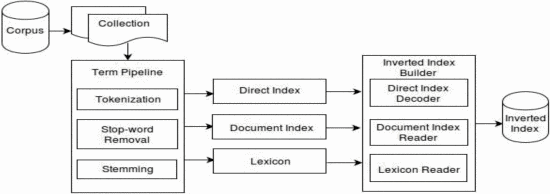
\includegraphics[width=\textwidth]{data-indexing.png}
    \caption{Data Indexing Process \cite{7830087}}
    \label{fig:data-indexing}
\end{figure}

With respect to information retrieval and recommendation system, data indexing has the following benefits:
\begin{itemize}
    \item improves performance in retrieving relevant documents
    \item optimizes the speed of the information retrieval system.
    \item helps to keep the data unique and drop the duplicates
    \item text-based indexes make it easier to search large string values, compared to conventional database approaches.
\end{itemize}

Considering the problem we are solving, data indexing is one of the crucial parts of the implementation strategy. In information retrieval or recommendation systems, latency for fetching the results, the efficiency of results, and relevancy of results for a given problem play the major part of the solution. All these tasks can be easily managed if the data is indexed in an efficient manner. 

\subsection{Elasticsearch and Apache Lucene architecture}
Elasticsearch is built on top of Apache Lucene and uses Lucene indexes. The concept of an inverted index is used while forming an index in Elasticsearch. The inverted index is created by mapping of terms to documents and their position in documents in the form of dictionary \cite{alex2013elastic}.
The dictionaries are sorted, so it's easier to find terms and hence the related documents. Opposite for this is a forward index, where the terms are related to specific documents, which is quite slow in search operations. Hence, an inverted index is used in forming the Elasticsearch index.

For a search operation with multiple terms, it is done by looking up all the terms and their respective occurrences, and the final results are comprised are some form of an aggregate of these results.
The main logic for search operation is, to find the respective terms, then the matching occurrences,  positions and consequently the documents. 

An Elasticsearch index is crated with one or more shards, that can have zero or more replicas. Each shard in an individual Lucene index. Thus, Elasticsearch index is made up of multiple Lucene indexes, which are made up of multiple index segments \cite{alex2013elastic}. A search operation in Elasticsearch index is executed on all the shards, and consequently all the segments and finally merged to give the output. A similar process is followed when multiple indexes are searched. It can also be thought as searching two indexes with one shard is same as searching one index with two shards, in both the cases two Lucene indexes are searched. Elasticsearch is also very flexible and provides options to optimize results, by providing options to define Elasticsearch indexes, which shards(and replicas), the search is directed to. Also, there are options to define index patterns, index aliases, document and search routes, data partitioning and data flow strategies. Figure \ref{fig:elasticsearch-architecture} summarizes this concept and shows the Elasticsearch architecture.

\begin{figure}
    \centering
    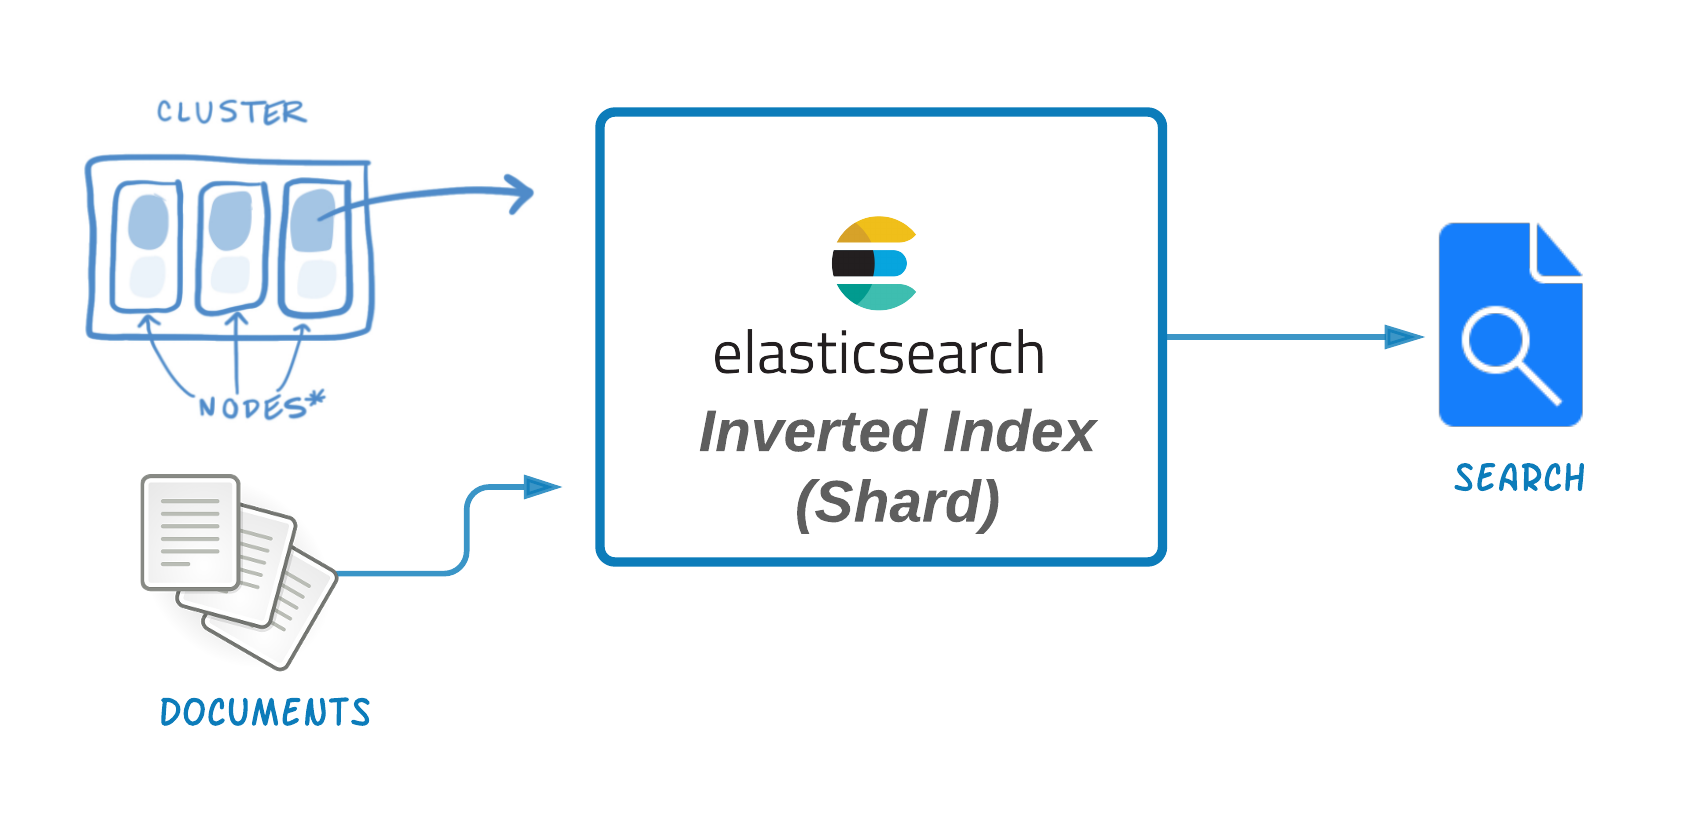
\includegraphics[width=120mm,scale=0.5]{elastic-architecture.png}
    \caption{Elasticsearch Architecture}
    \label{fig:elasticsearch-architecture}
\end{figure}

\subsection{Our implementation in Elasticsearch}
We have used Python and Elasticsearch to manage this task of data indexing. Since Elasticsearch is developed for the purpose of text-based retrieval system, so the major task of efficient indexing is done by it's internal processing. The python script takes care of the data collection, preprocessing and feeding the Elastic server with the data in the right format and remaining part of indexing is done by Elasticsearch. Figure \ref{fig:elasticsearch-architecture} explains the architecture for data indexing process. Once the data is indexed, it is shown as key-value pairs and also retrieved in the same key-value manner (as shown in Figure \ref{fig:citeulike-dataset}). 


The first index for all three datasets is created with the same mapping structure as given in the JSON files. The regular indexing in Elasticsearch stores the term with standard metrics. An important part to note is, all the metrics such as term frequency, document frequency, document length, average document length, etc. are calculated at the time of indexing itself and stored as index metadata. This also plays a significant role in document retrieval since term weights are just fetched from the metadata instead of calculating it at the moment. 

\section{Term Age Calculation and Indexing}
We have created three indexes for every dataset. First is the standard index with all standard metric as explained in the last section. For the second index, we add time normalized term weight factor or the term age to be stored along with other metrics. For calculating the term age, the following steps are done:
\begin{itemize}
    \item Iterate over the IDs stored in the first index and fetch the main article text
    \item Consider the article text of the document and split it into individual words. 
    \item For each of this word, get the origin year that is the year of the first occurrence of this word from etymonline.com.
    Figure \ref{fig:etymonline} shows the search results from the site and \textit{"1660"} is the considered as year of origin for this searched term \textit{"monologue"}.
    \begin{figure}[h!]
    \centering
    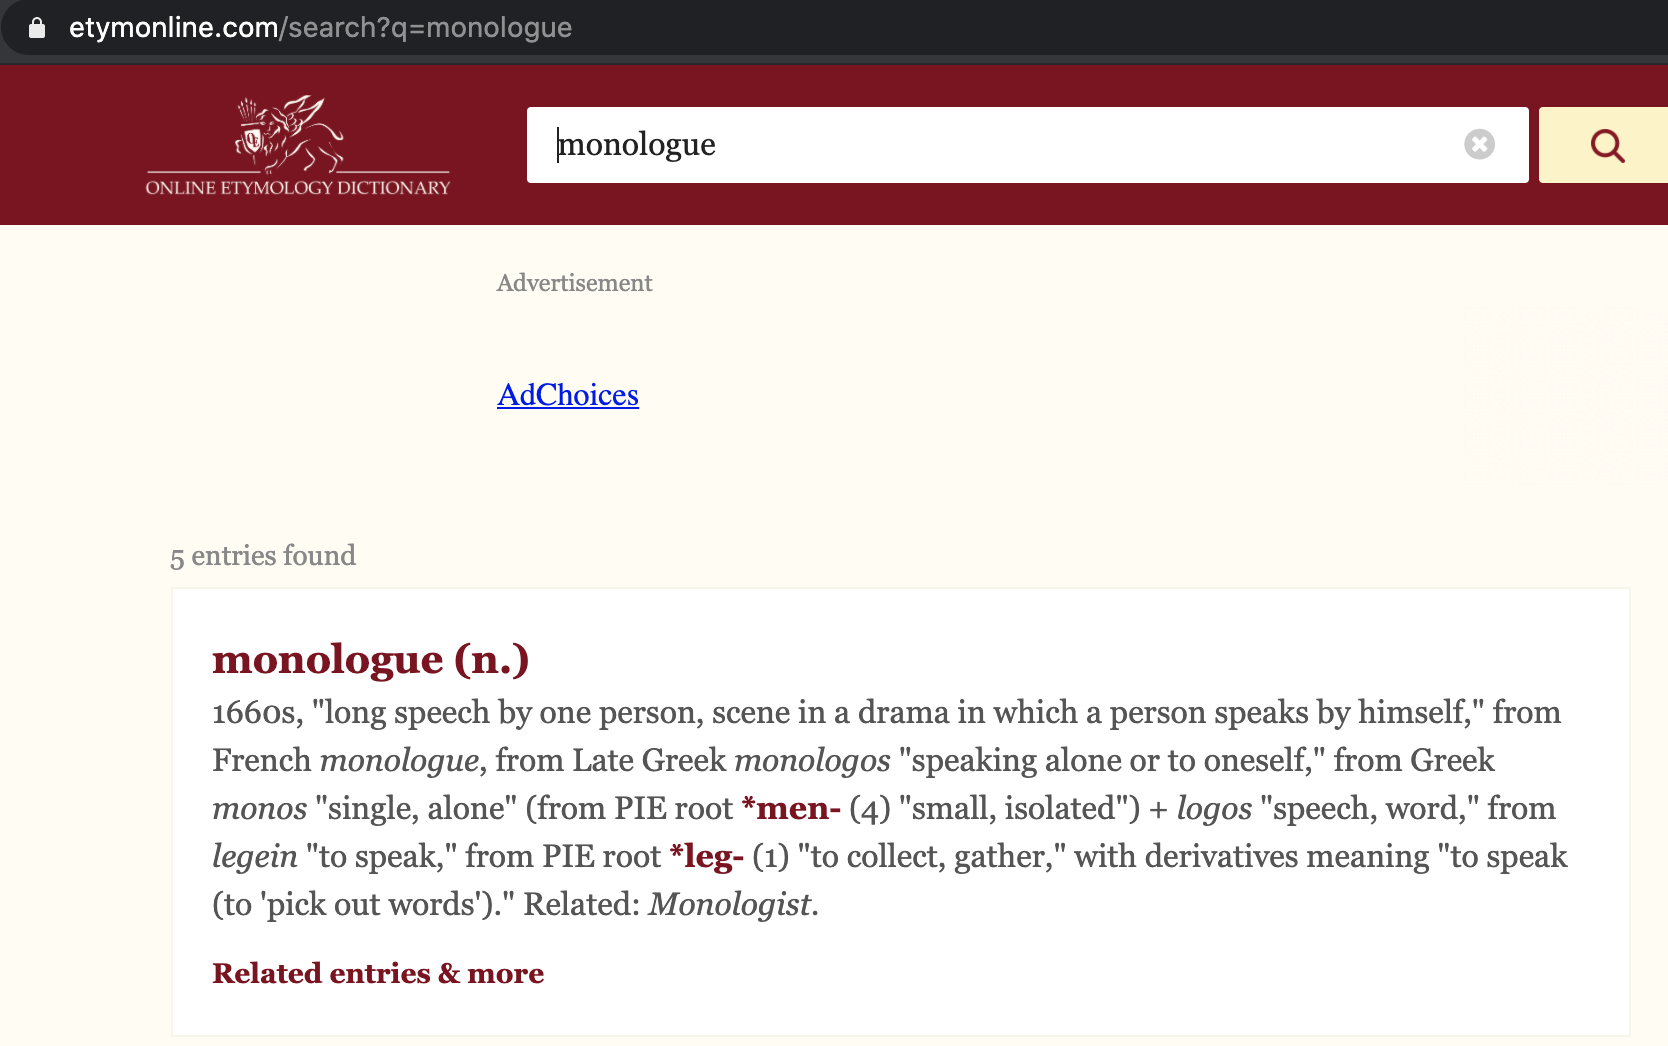
\includegraphics[width=140mm,scale=0.7]{Etymonline.png}
    \caption{Search results from Etymonline}
    \label{fig:etymonline}
    \end{figure}
    \item Calculate the difference in the number of years from the year of the first occurrence, to the current year. We have assumed the base year for our corpus to be 2017(TREC News), 2015(Web AP) and 2019(CiteULike) since that is the year of latest publications. This has been done for uniform term weighting across the corpus and to get the metric unit as documents per year.
    \item Now we fetch the document frequency, $df_{w,D}$ for a specific term $w$ and divide the document frequency with the year difference, as explained in chapter 4. 
    Since the value is relatively large, we have taken its logarithm value to normalize this term. Also, to avoid divide by zero error in cases when the term is newly devised and origin year is the same as the current year, we have added one to the denominator.
    \item Finally, the absolute value of the calculation done in the last step is the term age parameter and is calculated for every term in the article text. 
\end{itemize}

Once we have calculated the term age, we append this along with the terms using a separator. And the newly created article text is indexed in the form of payload index. Since the term age parameter does not have any standard column designated for it, we store it as payloads in the index and later use it in retrieval and relevance score calculation. Updated document text looks like this: \textit{“Americans|5.432 to|0.000 rate|5.466 their|1.080 ideology|3.303 on|0.000 a|0.000 scale|3.455 of|0.000 1|0.000 to|0.000 5|0.000.” }
An important part to note is, that not every term is given a term weight, this happens for a couple of reasons. First, if the origin year could not be traced for the term, this usually happens for proper nouns. Second, if the terms are most frequently used terms such as articles, prepositions, etc., that have a high document frequency value and in result might bias the results of the search query. Figure \ref{fig:payload-index} shows the mapping structure of a payload index, highlighting the term\_vector and analyzer fields showing the added analyzer for payloads.

\begin{figure}[h!]
    \centering
    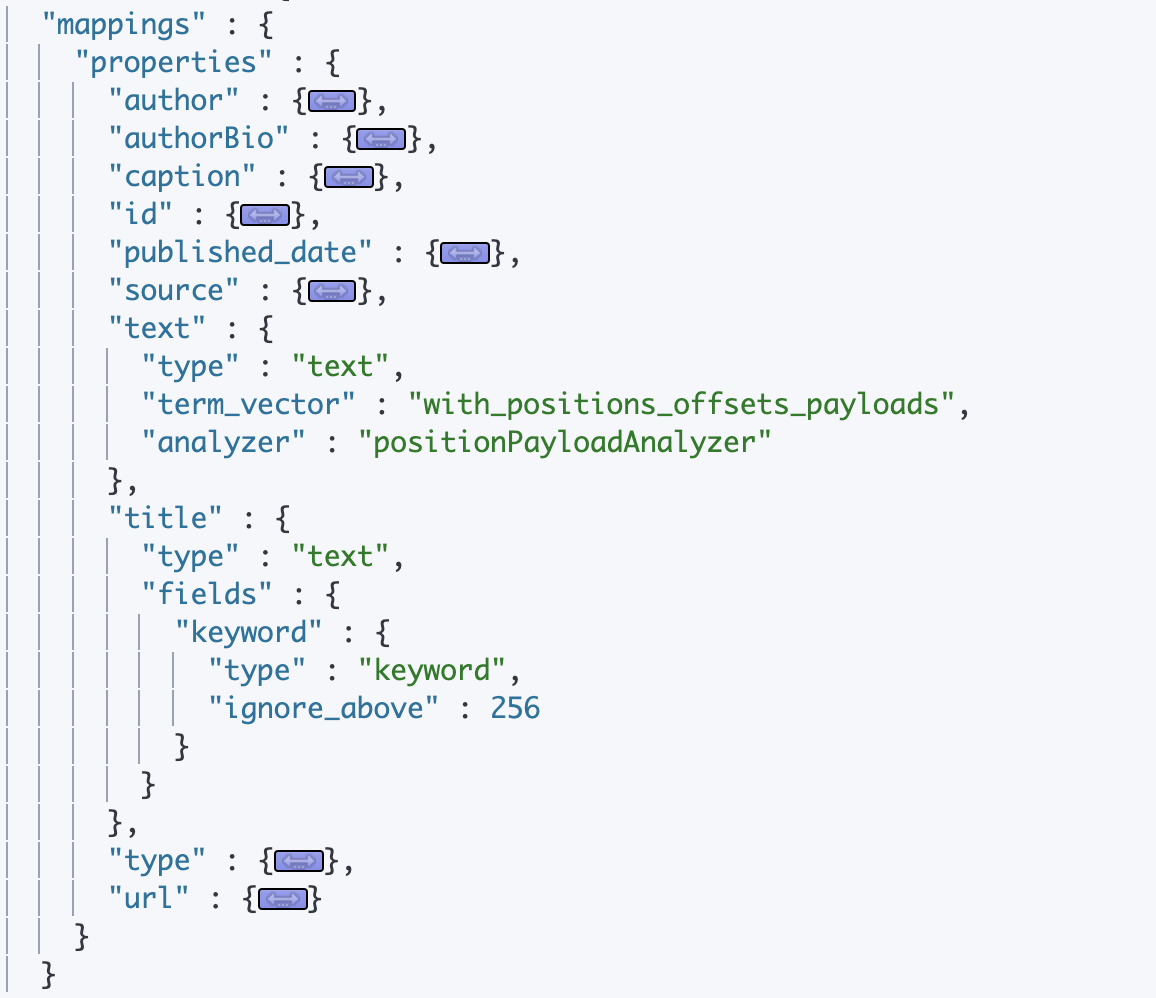
\includegraphics[width=120mm,scale=0.5]{payload-index.png}
    \caption{Payload Index Mapping Structure}
    \label{fig:payload-index}
\end{figure}

\section{USE based Payload Indexing}
For standard term weighting schemes, the relevant documents that are retrieved are based on the most number of term matches with the input query. However, to improve the search results, there are cases when the number of matching terms are less but still, the document might be relevant to the input query considering the semantic context. To overcome this issue and improve the performance of search engine or recommendation system, text embedding models are used, that encodes the text or sentence into a high dimensional numeric vector. These vector representations are developed in a way to consider the linguistic context of the terms into consideration. 

For a good text embedding model, different directions of the vector are coupled with different contexts of the same term. For example, the vector for the term "Canada", will be close to "France" or "French" in one direction and close to "Vancouver" in another direction \cite{julie2019USE}.

Mainly text embedding models focus on the word embedding and encode only the word into a dense vector. However, recently, some advance researches have also started to focus on longer texts such as sentence and try to capture the essence of the sentence into the dense vector. This is usually done with the help of neural network architectures focusing on the semantic context for the terms and sentences. Various advanced embedding models such as  Universal Sentence Encoder (USE) \cite{RN32}, Google’s BERT  \cite{DBLP:journals/corr/abs-1810-04805}, InferSent \cite{DBLP:journals/corr/ConneauKSBB17}, etc. are used for this purpose.


In our research, we have used Universal Sentence encoder model and created an index to store the dense vectors as well as the term age payloads. We have used a pre-trained Tensorflow model to form the dense vectors \cite{google2018use}. We use the following method to create a USE based index :
\begin{itemize}
    \item Iterate over the IDs stored in the first index and fetch the main article text.
    \item Main article text is run through a pre-trained Tensorflow model, creating a 512 dimension vector for the main text.
    \item Term age parameter is calculated in the same way as explained in the last section
    \item Same model is used to compute the dense vector for input query at the time of text retrieval.
\end{itemize}
Figure \ref{fig:architecture} shows the high-level architecture of the created indices, and search application.
Figure \ref{fig:use-index-mapping} shows the mapping structure of USE based index highlighting thee dense vector of 512 dimensions.
\begin{figure}
    \centering
    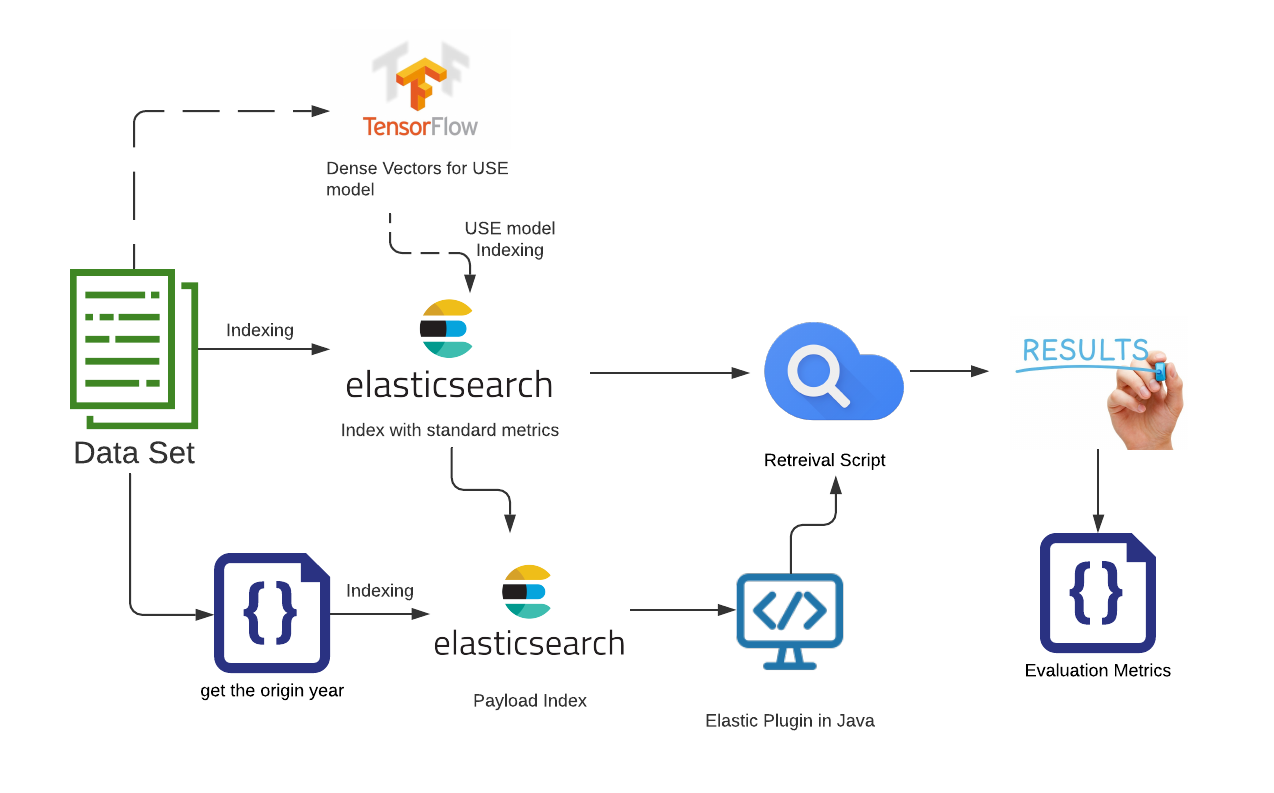
\includegraphics[width=140mm,scale=0.7]{System Architecture thesis.png}
    \caption{System Architecture}
    \label{fig:architecture}
\end{figure}

\begin{figure}[h!]
    \centering
    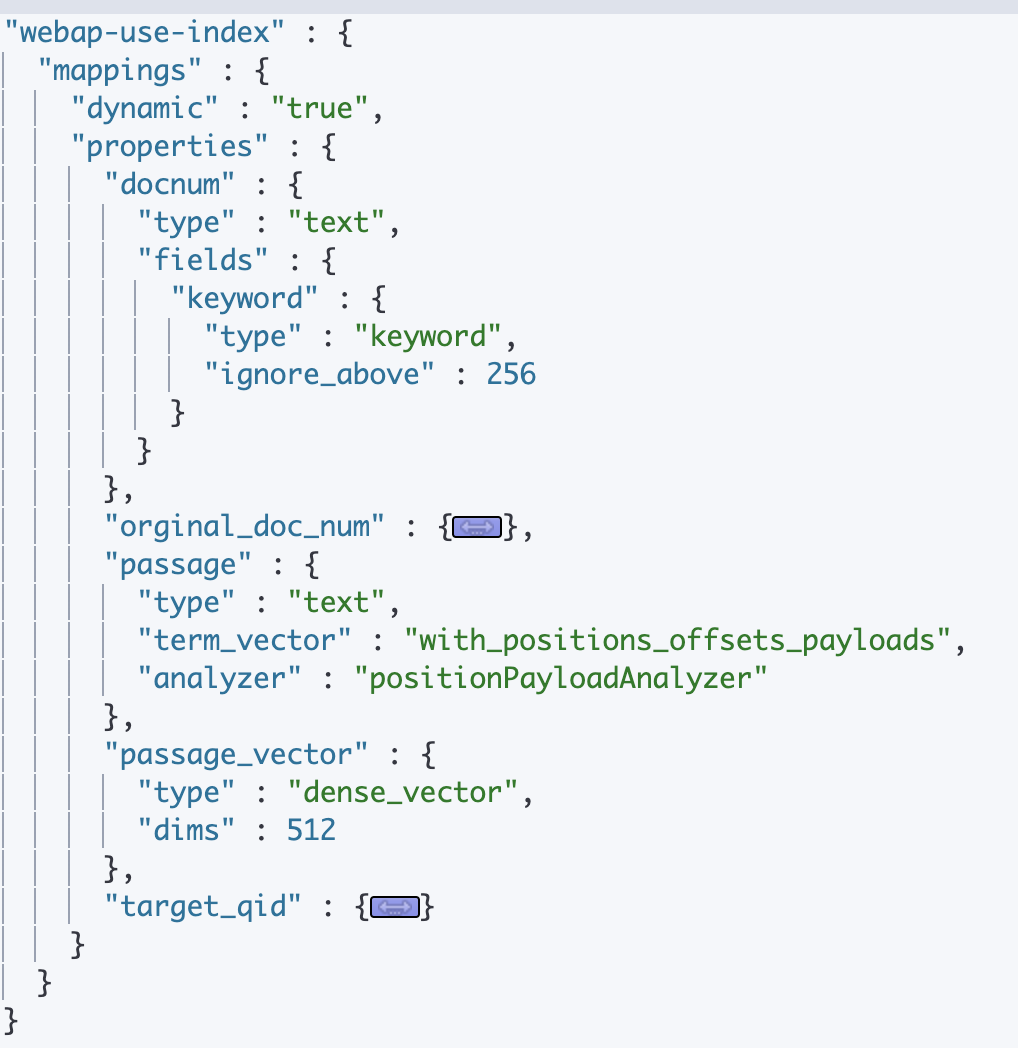
\includegraphics[width=120mm,scale=0.4]{use-index.png}
    \caption{USE based payload Index mapping}
    \label{fig:use-index-mapping}
\end{figure}

\section{Implementing Relevance Score calculation}
We have used Elasticsearch to create all three different indices for our datasets. Since Elasticsearch is built on top of Apache Lucene, that uses multiple parameters for score calculation. To have a uniform comparison with the baseline models we have implemented two different plugins. The first one just fetches standard metrics such as TF, IDF, Document length, etc. to calculate the relevance scoring and retrieves the results. The second plugin scores based on the calculated term weight parameter along with the standard metrics. These plugins are developed in Java and based on Apache Lucene plugins library. These plugins are then added into the Elasticsearch installation and also specified while indexing documents. Finally, we compare the results retrieved for the given set of queries from both these executions to our ground truth results. 

\subsection{Implementing Time Normalized TF-IDF(tTF-IDF)}
For standard TF-IDF model, it is based on just two metrics, Term frequency and inverse document frequency. These metrics are already stored in the metadata of the index are just fetched directly while retrieving documents. The formula for TF-IDF is given in equation \ref{eq:5.4}.
\begin{equation} \label{eq:5.4}
        wt_{w,d} = tf_{w,d}*log(\frac{N}{df_{w,d}})   
\end{equation}  
We fetch the results from the first index using this standard metric calculation and forms the first set of our results for the given input queries. For second set of results, we fetch the results based on our extended version of formula given in equation \ref{eq:5.5}. This is titled as tTF-IDF, where extra t stands for temporal dimension added to the existing formula. The term age parameter $t_{w,D}$ is stored as the term payload in the documents metadata. We leverage this metadata in our plugin to formulate this and calculate the relevance scores for the documents retrieved.
\begin{equation} \label{eq:5.5}
        wt_{w,d} = t_{w,D}*tf_{w,d}*log(\frac{N}{df_{w,d}})   
\end{equation} 
The results retrieved by using this updated formula, forms our second set of results. We have then compared the first and second set of results based on the precision, recall, F1 and NDCG metrics discussed in detail in chapter 7.

\subsection{Implementing Time Normalized BM25(tBM25)}
BM25 model is also based on term frequency and inverse document frequency, but the calculation logic for both these metrics is different from the standard TF-IDF model. IDF calculation is mainly the same, with just an added 1 in the denominator to avoid divide by zero exception. For TF, there are some added metrics of field length and average field length that are used. The term weight calculation is shown in equation \ref{eq:5.6}. 

\begin{equation} \label{eq:5.6}
    wt_{w,d} = \sum_{i}^{n}IDF(q_{i}) * \frac{f(q_{i},D)*(k1+1)}{f(q_{i},D)+k1*(1-b+b*\frac{fieldLen}{avgFieldLen})}
\end{equation}
First set of results for BM25 are fetched using this standard calculation. For second set of results, we fetch the results based on our extended version of formula given in \ref{eq:5.7}. This is titled as tBM25, where extra t stands for temporal dimension added to the existing formula. The term age parameter $t_{w,D}$ is stored as the term payload in the documents metadata. We leverage this metadata in our plugin to formulate this and calculate the relevance scores for the documents retrieved.
\begin{equation} \label{eq:5.7}
    wt_{w,d} = \sum_{i}^{n} t_{w,D}*IDF(q_{i}) * \frac{f(q_{i},D)*(k1+1)}{f(q_{i},D)+k1*(1-b+b*\frac{fieldLen}{avgFieldLen})}
\end{equation}

\subsection{Implementing Time Normalized Universal Sentence Encoder(tUSE)}
For a USE based model along with text similarity search, we have used cosine similarity function. Cosine similarity is already integrated in Elasticsearch and we leverage the same while getting the results. For this model, the input text query is first run through the same pre-trained sentence embedding model that produces a numeric vector. Now, to calculate the relevance score, we calculate the vector similarity between the input vector and the dense vector of the indexed documents. Cosine similarity calculates the angle $\theta$ between the two given vectors. This formulation is given in \ref{eq:5.8}.
\begin{equation} \label{eq:5.8}
    \cos \theta = \frac{\sum_{1}^{n} \vec a_{i}b_{i}}{\sqrt{\sum_{1}^{n} \vec a_{i}^2}\sqrt{\sum_{1}^{n} \vec b_{i}^2}}
\end{equation}
Some of the example, showing how this model return results are:
\begin{itemize}
    \item "zipping files" will also return results like "compression of files"
    \item "convert int to double" will also return results like "translate int to float numbers"
\end{itemize}
Although, there is not a strong overlap of terms in the input and output, still the results are considered relevant based on the semantics.

This forms the standard first set of results for our given input queries. As done in the previous models, we multiply the term age factor(stored in the metadata payload) in the standard calculation to get the tUSE formula as shown in equation \ref{eq:6.9}.
\begin{equation} \label{eq:6.9}
    \cos \theta = t_{w,D}*\frac{\sum_{1}^{n} \vec a_{i}b_{i}}{\sqrt{\sum_{1}^{n} \vec a_{i}^2}\sqrt{\sum_{1}^{n} \vec b_{i}^2}}
\end{equation}


\section{Key challenges}
In implementing and formulating this research project, we encountered some challenges listed below:
\begin{itemize}
    \item Finding an openly available ground truth dataset that matches up requirements was challenging. There are many text-based datasets available on the web, but a lot less with the defined gold standard. Even for the available ones, finding out the temporal context and how to apply it was challenging.
    \item Although Elasticsearch is open source and used in multiple research and production environments, there is still very less information available for defining payload index and how to use its scoring methodology. Figuring out the way to include time factor along with the index was one of the major roadblocks in implementing this research. We tried multiple methods such as using term age as boost parameter while querying, indexing term age as a separate dense vector field in the index, using a script score and function score methods in elasticsearch.  But none of them sufficed to our research statement.
    \item The existing libraries in Python for Precision and NDCG do not give out the correct results as per the metric definitions. For example, on using scikit-learn's NDCG function returns the NDCG value as 1, even when no results match in the result set. To overcome this issue, we implemented custom-built methods for computing NDCG and precision for our algorithm and validated it giving the correct results as per the metric definition.
    
    
\end{itemize}
